\begin{frame}
\frametitle{Algebraic Topology}
\begin{itemize}
\item<1-> We need a way show that no deformation exists between two spaces.
\item<2-> This is a very difficult problem.
\item<3-> We need a workaround.
\end{itemize}
\end{frame}

\begin{frame}
\frametitle{Algebraic Topology}
\begin{itemize}
\item<1-> Abstract Algebra is the study of different {\color{red}algebraic structures}.
	\begin{itemize}
	\item<2-> $\mathbb{R}$
	\item<2-> $\mathbb{Q}$
	\item<2-> $\mathbb{Z}$
	\item<2-> $\mathbb{Z}/p$
	\end{itemize}
\item<3-> Trick: Assign to each topological space algebraic structures in a clever way. 
\item<4-> If two spaces have different structures, then they are not `the same'.
\end{itemize}
\end{frame}


\begin{frame}
\frametitle{Algebraic Topology}
\begin{itemize}
\item<1-> One of the most popular ways to assign an algebraic structure to a topological space $X$ is \textbf{homology}.
\item<2-> The $n$-th homology group, denoted $H_n(X; \mathbb{Z})$, is a very useful algebraic structure.
\item<3-> The $n$-th \textbf{Betti number} $\beta_n$ counts the number of $n$-dimensional holes in a space.
\item<4-> The $n$-th \textbf{Betti number} $\beta_n$ counts the number of $\mathbb{Z}$-summands in $H_n(X;\mathbb{Z})$.
\end{itemize}
\end{frame}

\begin{frame}
\frametitle{Algebraic Topology}
\[ \beta_j = \begin{cases} 
      	1 & j = 0, 1 \\
      	0 & j \neq 1 
   \end{cases}
\]
%\begin{center}
%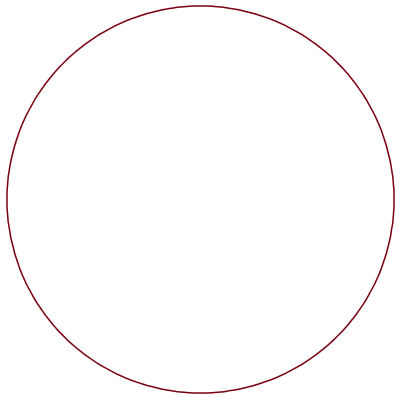
\includegraphics[scale=0.3]{S1}
%\end{center}
\end{frame}

\begin{frame}
\frametitle{Algebraic Topology}
\[ \beta_j = \begin{cases} 
      1 & j = 0, 2 \\
      0 & j \neq 2 
   \end{cases}
\]
%\begin{center}
%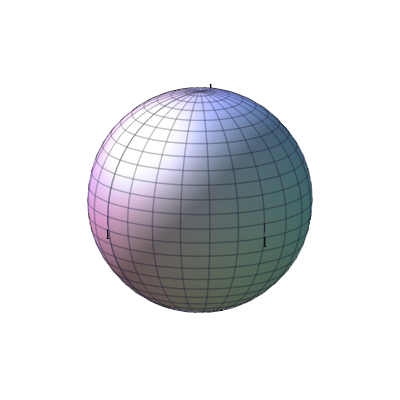
\includegraphics[scale=0.5]{S2}
%\end{center}
\end{frame}

\begin{frame}
\frametitle{Algebraic Topology}
\[ \beta_j = \begin{cases} 
      2 & j = 0, 1 \\
      0 & j \neq 2 
   \end{cases}
\]
%\begin{center}
%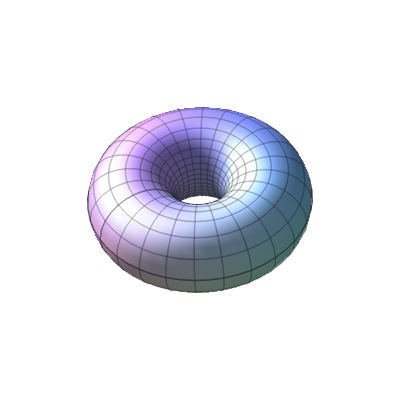
\includegraphics[scale=0.5]{Torus}
%\end{center}
\end{frame}

\begin{frame}
\frametitle{Algebraic Topology}
\begin{itemize}
\item<1-> {\fontsize{70}{80}\selectfont \textsf{  A  }} $\beta_1 = 1$
\item<2-> {\fontsize{70}{80}\selectfont \textsf{  B  }} $\beta_1 = 2$

So A and B are not the same in the eyes of a topologist.
\end{itemize}

\end{frame}